%%%%%%%%%%%%%%%%%%%%%%%%%%%%%%%%%%%%%%%%%
% Beamer Presentation
% LaTeX Template
% Version 1.0 (10/11/12)
%
% This template has been downloaded from:
% http://www.LaTeXTemplates.com
%
% License:
% CC BY-NC-SA 3.0 (http://creativecommons.org/licenses/by-nc-sa/3.0/)
%
%%%%%%%%%%%%%%%%%%%%%%%%%%%%%%%%%%%%%%%%%

%----------------------------------------------------------------------------------------
%	PACKAGES AND THEMES
%----------------------------------------------------------------------------------------

\documentclass{beamer}

\mode<presentation> {

% The Beamer class comes with a number of default slide themes
% which change the colors and layouts of slides. Below this is a list
% of all the themes, uncomment each in turn to see what they look like.

\usetheme{default}
%\usetheme{AnnArbor}
%\usetheme{Antibes}
%\usetheme{Bergen}
%\usetheme{Berkeley}
%\usetheme{Berlin}
%\usetheme{Boadilla}
%\usetheme{CambridgeUS}
%\usetheme{Copenhagen}
%\usetheme{Darmstadt}
%\usetheme{Dresden}
%\usetheme{Frankfurt}
%\usetheme{Goettingen}
%\usetheme{Hannover}
%\usetheme{Ilmenau}
%\usetheme{JuanLesPins}
%\usetheme{Luebeck}
%%\usetheme{Madrid}
%\usetheme{Malmoe}
%\usetheme{Marburg}
%\usetheme{Montpellier}
%\usetheme{PaloAlto}
%\usetheme{Pittsburgh}
%\usetheme{Rochester}
%\usetheme{Singapore}
%\usetheme{Szeged}
%\usetheme{Warsaw}

% As well as themes, the Beamer class has a number of color themes
% for any slide theme. Uncomment each of these in turn to see how it
% changes the colors of your current slide theme.

%\usecolortheme{albatross}
%\usecolortheme{beaver}
%\usecolortheme{beetle}
%\usecolortheme{crane}
%\usecolortheme{dolphin}
%\usecolortheme{dove}
%\usecolortheme{fly}
%\usecolortheme{lily}
%\usecolortheme{orchid}
%\usecolortheme{rose}
%\usecolortheme{seagull}
%\usecolortheme{seahorse}
%\usecolortheme{whale}
%\usecolortheme{wolverine}

%\setbeamertemplate{footline} % To remove the footer line in all slides uncomment this line
%\setbeamertemplate{footline}[page number] % To replace the footer line in all slides with a simple slide count uncomment this line

%\setbeamertemplate{navigation symbols}{} % To remove the navigation symbols from the bottom of all slides uncomment this line
}

\usepackage{graphicx} % Allows including images
\usepackage{booktabs} % Allows the use of \toprule, \midrule and \bottomrule in tables

%--------------------------
%bibliography
\usepackage[numbers]{natbib} %[numbers]
\renewcommand\bibname{\refname} %renames Bibliography -> References
%fixes underscore error in bibliography urls
\usepackage{url}
\let\harvardurl\url

%eq scaling
\newcommand*{\Scale}[2][4]{\scalebox{#1}{$#2$}}%
\newcommand*{\Resize}[2]{\resizebox{#1}{!}{$#2$}}%

%--------------------------

%----------------------------------------------------------------------------------------
%	TITLE PAGE
%----------------------------------------------------------------------------------------

\title{On the Hierarchy Classes of Finite Ultrametric Automata} % [Short title] The short title appears at the bottom of every slide, the full title is only on the title page

\author{Rihards Kri\v{s}lauks} % Your name
\institute[LU] % Your institution as it will appear on the bottom of every slide, may be shorthand to save space
{
University of Latvia Faculty of Computing \\ % Your institution for the title page
%\medskip
%\textit{john@smith.com} % Your email address
}
\date{\today} % Date, can be changed to a custom date

\begin{document}

\begin{frame}
\titlepage % Print the title page as the first slide
\end{frame}

\iffalse
\begin{frame}
\frametitle{Overview} % Table of contents slide, comment this block out to remove it
\tableofcontents % Throughout your presentation, if you choose to use \section{} and \subsection{} commands, these will automatically be printed on this slide as an overview of your presentation
\end{frame}
\fi
%----------------------------------------------------------------------------------------
%	PRESENTATION SLIDES
%----------------------------------------------------------------------------------------

%------------------------------------------------
\section{First Section} % Sections can be created in order to organize your presentation into discrete blocks, all sections and subsections are automatically printed in the table of contents as an overview of the talk
%------------------------------------------------

\subsection{Subsection Example} % A subsection can be created just before a set of slides with a common theme to further break down your presentation into chunks

\begin{frame}
\frametitle{Ultrametric finite automata and ultrametric Turing machines}
\begin{itemize}
	\item Introduced by \cite{Freivalds2012}
	\item "[..] using $p$-adic numbers is not merely one of many possibilities to generalize the definition of deterministic algorithms but rather the only remaining possibility not yet explored."
\end{itemize}
\end{frame}

%------------------------------------------------
\begin{frame}
\frametitle{Probabilities}
\begin{itemize}
\item Pascal and Fermat believed that every event of indeterminism can be described by a real number between 0 and 1 called probability.
\item Quantum physics introduced a description in terms of complex numbers called amplitude of probabilities and later in terms of probabilistic combinations of amplitudes most conveniently described by density matrices.
\item String theory \cite{V.S.Vladimirov1995}, chemistry \cite{Kozyrev2006} and molecular biology \cite{Dragovich2009} have introduced p-adic numbers to describe measures of indeterminism.
\end{itemize}
\end{frame}

%------------------------------------------------
\begin{frame}
\frametitle{$p$-adic numbers}
\begin{itemize}
	\item For any given prime $p$ the field $\mathbb{Q}_p$ of $p$-adic numbers is a completion of rational numbers.
	%TODO extends the ordinary arithmetic of the rational numbers in a way different from the extension of the rational number system to the real and complex number systems
	\item $p$-adic numbers cannot be linearly ordered.
	\item In 1916 Alexander Ostrowski 
proved that any non-trivial absolute value on the rational numbers $\mathbb{Q}$ is equivalent to either the usual real absolute value or a $p$-adic absolute value.
	\item Helmut Hasse's local-global principle
 states that certain types of equations have a rational solution if and only if they have a solution in the real numbers and in the $p$-adic numbers for each prime $p$.
 	%TODO vai ieprieksejo vajag?
\end{itemize}
\end{frame}

%------------------------------------------------
\begin{frame}
\frametitle{Motivation for our paper}
\begin{itemize}
	\item \citep{KasparsBalodis2013} showed that regularized ultrametric automata recognize exactly the set of regular languages.
	\item \citep{Holzer2009, Yao1978, Monien1980, Macarie1995} show results for deterministic, nondeterministic and probabilistic multihead finite automata in the two-way and one-way cases.
\end{itemize}
\end{frame}


%------------------------------------------------
\begin{frame}
\frametitle{Definitions -- $p$-norm}
For every non-zero rational number $\alpha$ there exists a unique prime factorization $\alpha = \pm 2^{\alpha_2}3^{\alpha_3}5^{\alpha_5}7^{\alpha_7} \cdots$ where $\alpha_i \in \mathbb{Z}$.
%\begin{definition}

The $p$-adic absolute value (also called the \textbf{$p$-norm}) of a rational number $\alpha = \pm 2^{\alpha_2}3^{\alpha_3}5^{\alpha_5}7^{\alpha_7} \cdots$ is 
\[
\|\alpha\|_p = \begin{cases}
p^{-\alpha_p}, &\textrm{if } \alpha \neq 0 \\
0, &\textrm{if } \alpha = 0.
\end{cases}
\]
%\end{definition}
\end{frame}

%------------------------------------------------
\begin{frame}
\frametitle{Definitions -- ultrametric automata}
A finite one-way $p$-ultrametric one-head automaton  ($1\mathit{u_pfa}$ or $1\mathit{u_pfa}(1)$) is a sextuple
$\langle S, \Sigma, s_0, \delta, Q_A, Q_R \rangle$ where
\begin{itemize}
  \item $S$ is a finite set---the set of states,
  \item $\Sigma$ is a finite set ($\$ \notin \Sigma$)---input alphabet,
  \item $s_0:S \rightarrow \mathbb{Q}_p$ is the initial amplitude distribution,
  \item $\delta: \left( \Sigma \cup \left\{ \$ \right\} \right) \times S \times S \rightarrow \mathbb{Q}_p$ is the transition function,
  \item $Q_A, Q_R \subseteq S$ are the sets of accepting and rejecting states, respectively.
\end{itemize}

The amplitude distribution after processing the $i$-th symbol is denoted as $s_i$, with
$s_i(y) = \sum_{x \in S}{s_{i-1}(x) \cdot \delta \left( w_i, x, y \right) }$ for every $y \in S$.

If $\sum_{x \in Q_A}{\left\| s_{n+1}(x) \right\|_p} > \sum_{x \in Q_R}{\left\| s_{n+1}(x) \right\|_p}$, then the word $w$ is said to be accepted, otherwise---rejected.

\end{frame}
%-----------------------------------------
\begin{frame}
\frametitle{Results -- $1\mathit{u_pfa}(1)$ vs $1\mathit{nfa}(k)$}
Let $n={k\choose 2}+1$.
\[
L_k = \left\{ w_1 1 w_2 1 \ldots 1 w_{2n} \middle|
		w_i \in \left\{ 0^m | m \geq 1 \right\} \wedge
		w_i = w_{2n-i+1} 
		 \right\}.
\]
\begin{theorem}
\begin{enumerate}
	\item For every prime $p$ there exists a $1\mathit{u_pfa}(1)$ that recognizes $L_k$,
	\item $L_k$ cannot be recognized by any $1\mathit{nfa}(k)$.
\end{enumerate}
\end{theorem}
%-----------------------------------------------
\end{frame}
\begin{frame}
\frametitle{Proof -- used constructions}
\small
\begin{figure}
\centering
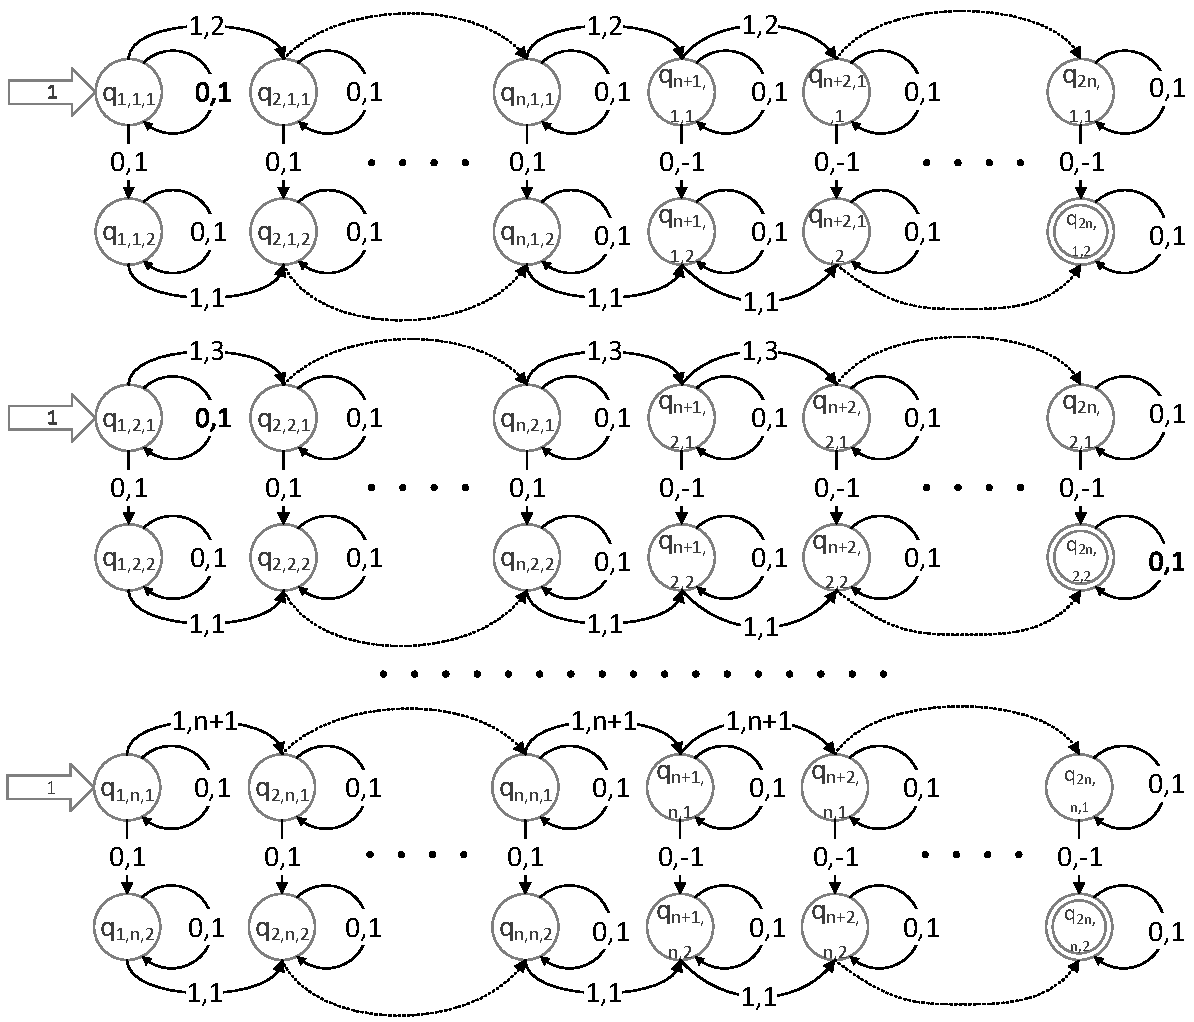
\includegraphics[width=0.6\textwidth]{Img/1pfa.pdf}
\caption{Automaton for recognizing $0^n10^m10^h1 \cdots 10^h10^m10^n$. Double-circled states are rejecting. Large arrows with labels in them show the amplitude distribution when the automaton starts. Small labelled arrows show transitions. A label $(a, b)$ indicates that if the automaton reads $a$, transition with amplitude $b$ should be made.}
\label{fig:1pfa}
\end{figure}
\end{frame}
%------------------------------------------------
\begin{frame}
\frametitle{Proof -- used constructions}
\tiny
\begin{gather*}
%\allowdisplaybreaks
	\begin{cases}
		a_1 + a_2 \cdot 2 + a_3 \cdot 2^2 + \cdots + a_n \cdot 2^{n - 1} - a_{n+1} \cdot 2^{n - 1} - a_{n+2} \cdot 2^{n - 2} - \cdots - a_{2n} = 0 \\
		a_1 + a_2 \cdot 3 + a_3 \cdot 3^2 + \cdots + a_n \cdot 3^{n - 1} - a_{n+1} \cdot 3^{n - 1} - a_{n+2} \cdot 3^{n - 2} - \cdots - a_{2n} = 0\\
		% a_1 + a_2 \cdot 4 + a_3 \cdot 4^2 + \cdots + a_n \cdot 4^{n - 1} - a_{n+1} \cdot 4^{n - 1} - a_{n+2} \cdot 4^{n - 2} - \cdots - a_{2n} = 0\\
		\cdots \\
		\begin{split}
		a_1 + a_2 \cdot (n + 1) + a_3 \cdot (n + 1)^2 + \cdots + a_n \cdot (n + 1)^{n - 1} - a_{n+1} \cdot (n + 1)^{n - 1} \\
		\qquad- a_{n+2} \cdot (n + 1)^{n - 2} - \cdots - a_{2n} = 0\\
		\end{split}
	\end{cases}\\
\small
\intertext{rewriting}
\tiny
	\begin{cases}
		(a_1 - a_{2n}) + 2 \cdot (a_2 - a_{2n-1}) + 2^2 \cdot (a_3 - a_{2n-2}) + \cdots + 2^{n - 1} \cdot (a_n - a_{n+1}) = 0\\
		(a_1 - a_{2n}) + 3 \cdot (a_2 - a_{2n-1}) + 3^2 \cdot (a_3 - a_{2n-2}) + \cdots + 3^{n - 1} \cdot (a_n - a_{n+1}) = 0\\
		% (a_1 - a_{2n}) + 4 \cdot (a_2 - a_{2n-1}) + 4^2 \cdot (a_3 - a_{2n-2}) + \cdots + 4^{n - 1} \cdot (a_n - a_{n+1}) = 0\\
		\cdots \\
		\begin{split}
		(a_1 - a_{2n}) + (n + 1) \cdot (a_2 - a_{2n-1}) + (n + 1)^2 \cdot (a_3 - a_{2n-2}) + \cdots \\
		\qquad+ (n + 1)^{n - 1} \cdot (a_n - a_{n+1}) = 0\\
		\end{split}	
	\end{cases}
\end{gather*}

\end{frame}
%------------------------------------------------

\begin{frame}
\frametitle{Results -- two-way multi-head automata}
By $\widehat{C}$, we denote the subset of a language class $C$ containing only the words in the form $1^{2^n}, n \in \mathbb{N}$, more precisely  
$\widehat{C} = \left\{ L \in C | \forall x \in L \; \exists n \in \mathbb{N} : x = 1^{2^n} \right\}$
% $\widehat{C} = \left\{ h | h \in C \wedge \exists n \in \mathbb{N} : h = 1^{2^n} \right\}$\\

\begin{theorem} \label{atdalisana}
For every natural number $k$ and prime $p$:
\[
	\widehat{2\mathit{U_pFA}(k)} \subsetneqq \widehat{U_pTM}.
\]
\end{theorem}
We will construct a special $p$-ultrametric Turing machine with 2 tapes and $log$-space space complexity called $\mathcal{T}$. We will show that its recognized language cannot be recognized by a $p$-ultrametric automata with $k$ heads for any $k$.

\end{frame}
%------------------------------------------------

\begin{frame}
\frametitle{Proof -- used constructions}
Similarly, as in \citep{Macarie1995} and \citep{Monien1980}, in the following proofs we will use the function
$
	f_k : \left\{ 1^{2^n} | n \in \mathbb{N} \right\} \rightarrow \left\{ 1^{2^n} | n \in \mathbb{N} \right\} \textrm{, where } f_k( 1^{2^n}) = 1^{2^{k \cdot n}}
$.

When $f_k$ is applied to a language, we refer to the following function: $f_k(L) = \left\{ f_k(x) \middle| x\in L \right\}$.

\begin{lemma} \label{skaititaji}
For every language $L \in \widehat{U_pTM}$ that is recognized by a 2-tape $u_ptm$ in logarithmic space, there exists a natural number $u$ such that:
$
	f_u(L) \in \widehat{2\mathit{U_pFA}(3)}.
$
\end{lemma}
We will show how a $u_ptm$ denoted by $\mathcal{T}$ that recognizes $L$ can be transformed into a $u_ptm$ called $\mathcal{T'}$, which can then be replaced by a $p$-ultrametric $3$ register machine. From this, it easily follows that there exists a $2\mathit{u_pfa}(3)$ that recognizes a ``stretched"  variant of $L$, where stretching is done by $f_u$.

\end{frame}
%------------------------------------------------
\begin{frame}
\frametitle{Proof -- used constructions}
\begin{lemma} \label{reizinajums}
For all languages $L \in \widehat{U_pTM}$ and all $u, v \geq 1, u, v \in \mathbb{N}$:
$
	f_u(L) \in \widehat{2\mathit{U_pFA}(v)} \Rightarrow L \in \widehat{2\mathit{U_pFA}(u \cdot v)}.
$
\end{lemma}
\end{frame}
%------------------------------------------------
\begin{frame}
\frametitle{Definition}
\begin{lemma} \label{plus1}
For every language $L \in \widehat{U_pTM}$ and every $u > v > 1, u, v \in \mathbb{N}$:
\[
	f_{u+1}(L) \in \widehat{2\mathit{U_pFA}(v)} \Rightarrow f_u(L) \in \widehat{2\mathit{U_pFA}(v + 1)}.
\]
\end{lemma}
\end{frame}
%------------------------------------------------
\begin{frame}
\frametitle{Proof -- used constructions}
\begin{theorem}
For all $k \geq 2 \in \mathbb{N}$:
\[
	\widehat{2\mathit{U_pFA}(k)} \subsetneqq \widehat{2\mathit{U_pFA}(k + 1)}.
\]
\end{theorem}
We prove from the contrary by showing that if there exists such $h \geq 2$ that $\widehat{2\mathit{U_pFA}(h)} = \widehat{2\mathit{U_pFA}(h + 1)}$, it implies $\widehat{2\mathit{U_pFA}(h \cdot (h + 1))} = \widehat{U_pTM}$, which contradicts $\widehat{2\mathit{U_pFA}(k)} \subsetneqq \widehat{U_pTM}$.

\end{frame}
%------------------------------------------------


\begin{frame}
\frametitle{Bullet Points}
\begin{itemize}
\item Lorem ipsum dolor sit amet, consectetur adipiscing elit
\item Aliquam blandit faucibus nisi, sit amet dapibus enim tempus eu
\item Nulla commodo, erat quis gravida posuere, elit lacus lobortis est, quis porttitor odio mauris at libero
\item Nam cursus est eget velit posuere pellentesque
\item Vestibulum faucibus velit a augue condimentum quis convallis nulla gravida
\end{itemize}
\end{frame}

%------------------------------------------------

\begin{frame}
\frametitle{Blocks of Highlighted Text}
\begin{block}{Block 1}
Lorem ipsum dolor sit amet, consectetur adipiscing elit. Integer lectus nisl, ultricies in feugiat rutrum, porttitor sit amet augue. Aliquam ut tortor mauris. Sed volutpat ante purus, quis accumsan dolor.
\end{block}

\begin{block}{Block 2}
Pellentesque sed tellus purus. Class aptent taciti sociosqu ad litora torquent per conubia nostra, per inceptos himenaeos. Vestibulum quis magna at risus dictum tempor eu vitae velit.
\end{block}

\begin{block}{Block 3}
Suspendisse tincidunt sagittis gravida. Curabitur condimentum, enim sed venenatis rutrum, ipsum neque consectetur orci, sed blandit justo nisi ac lacus.
\end{block}
\end{frame}

%------------------------------------------------

\begin{frame}
\frametitle{Multiple Columns}
\begin{columns}[c] % The "c" option specifies centered vertical alignment while the "t" option is used for top vertical alignment

\column{.45\textwidth} % Left column and width
\textbf{Heading}
\begin{enumerate}
\item Statement
\item Explanation
\item Example
\end{enumerate}

\column{.5\textwidth} % Right column and width
Lorem ipsum dolor sit amet, consectetur adipiscing elit. Integer lectus nisl, ultricies in feugiat rutrum, porttitor sit amet augue. Aliquam ut tortor mauris. Sed volutpat ante purus, quis accumsan dolor.

\end{columns}
\end{frame}

%------------------------------------------------
\section{Second Section}
%------------------------------------------------

\begin{frame}
\frametitle{Table}
\begin{table}
\begin{tabular}{l l l}
\toprule
\textbf{Treatments} & \textbf{Response 1} & \textbf{Response 2}\\
\midrule
Treatment 1 & 0.0003262 & 0.562 \\
Treatment 2 & 0.0015681 & 0.910 \\
Treatment 3 & 0.0009271 & 0.296 \\
\bottomrule
\end{tabular}
\caption{Table caption}
\end{table}
\end{frame}

%------------------------------------------------

\begin{frame}
\frametitle{Theorem}
\begin{theorem}[Mass--energy equivalence]
$E = mc^2$
\end{theorem}
\end{frame}

%------------------------------------------------

\begin{frame}[fragile] % Need to use the fragile option when verbatim is used in the slide
\frametitle{Verbatim}
\begin{example}[Theorem Slide Code]
\begin{verbatim}
\begin{frame}
\frametitle{Theorem}
\begin{theorem}[Mass--energy equivalence]
$E = mc^2$
\end{theorem}
\end{frame}\end{verbatim}
\end{example}
\end{frame}

%------------------------------------------------

\begin{frame}
\frametitle{Figure}
Uncomment the code on this slide to include your own image from the same directory as the template .TeX file.
%\begin{figure}
%\includegraphics[width=0.8\linewidth]{test}
%\end{figure}
\end{frame}

%------------------------------------------------

\begin{frame}[fragile] % Need to use the fragile option when verbatim is used in the slide
\frametitle{Citation}
An example of the \verb|\cite| command to cite within the presentation:\\~

This statement requires citation \cite{p1}.
\end{frame}

%------------------------------------------------

\begin{frame}
\frametitle{References}
\footnotesize{
\begin{thebibliography}{99} % Beamer does not support BibTeX so references must be inserted manually as below
\bibitem[Smith, 2012]{p1} John Smith (2012)
\newblock Title of the publication
\newblock \emph{Journal Name} 12(3), 45 -- 678.
\end{thebibliography}
}
\end{frame}

%------------------------------------------------

\begin{frame}
\Huge{\centerline{The End}}
\end{frame}

%----------------------------------------------------------------------------------------

\end{document} 